\section{FrBu II.2 2}

\begin{tcolorbox}[width=\textwidth,
colback={shadecolor},
title={Question:},colbacktitle=white,coltitle=black]

    Let $\alpha : [0, \pi] \rightarrow \mathbb{C} $ be defined by
    $$\alpha(t) = e^{it}$$
    and $\beta : [0, 2] \rightarrow \mathbb{C} $ by

    \[
        \beta(t)=\left\{
        \begin{array}{lll}
            1 + t(-i-1) & \text{for } t \in [0,1]\\
            1 - t +i(t-2) & \text{for } t \in [1,2].
        \end{array}
        \right.
    \]

    Sketch $\alpha$, and $\beta$, and calculate

    $$ \int_{\alpha} \frac{1}{z} dz \text{ and } \int_{\beta} \frac{1}{z} dz.$$

\end{tcolorbox}

\answerBox{
Sketch of $\alpha$, and $\beta$:

\begin{figure}[H]
    \centering
%    \includegraphics[width=0.5\textwidth]{frbu212.png}
    \includegraphics[width=0.5\textwidth]{pics/frbu212.png}
%   \caption{}
\end{figure}

%$$ \int_{\alpha} \frac{1}{z} dz \text{ and } \int_{\beta} \frac{1}{z} dz.$$
Calculation of the integral along $\alpha$:
\begin{equation*}
    \begin{split}
        \int_{\alpha} \frac{1}{z} dz &= \int_{0}^{\pi} \frac{1}{e^{it}}i e^{it} dt\\
        & = \int_{0}^{\pi} i dt \\
        & = \left[ i t \right]_0^\pi \\
        & = \pi i
    \end{split}
\end{equation*}

Calculation of the integral along $\beta$:
\begin{equation*}
    \begin{split}
        \int_{\beta} \frac{1}{z} dz &=
    \end{split}
\end{equation*}

}